\documentclass{article}

\usepackage{graphicx}
\usepackage{subcaption}
\usepackage{setspace}
\usepackage[utf8]{inputenc}
\usepackage{polski}
\usepackage{apacite}



%name and stuff
\title{Autonomiczna Nawigacja Manipulatora Dwuręcznego z Wielokierunkową Bazą Mobilną}
\date{\today}
\author{Marcin Skrzypkowski}



\begin{document}
	
	
	%customizacja strony tytułowej
	\makeatletter
	\renewcommand{\maketitle}{\begin{titlepage}
		\begin{center}{\LARGE {\bf Wydział Elektroniki i Technik Informacyjnych}}\\
			\vspace{0.4cm}
			{\LARGE {\bf Politechnika Warszawska}}\\
			\vspace{0.3cm}
		\end{center}
		\vspace{5cm}
		\begin{center}
			{\bf \LARGE Pracownia Dyplomowa Inżynierska  1\\ sprawozdanie  \vskip 0.1cm}
		\end{center}
		\vspace{1cm}
		\begin{center}
			{\bf \LARGE \@title}
		\end{center}
		\vspace{2cm}
		\begin{center}
			{\bf \Large \@author \par}
		\end{center}
		\vspace*{\stretch{1}}
		\begin{center}
			{\bf  opiekun pracy: \\ dr inż. Wojciech Szynkniewicz\par}
		\end{center}
		\vspace*{\stretch{5}}
		\begin{center}
			\bf{\large{Warszawa, \@date\vskip 0.1cm}}
		\end{center}
		\end{titlepage}
}
\makeatother	


	

	\pagenumbering{gobble}
	\maketitle
	\newpage



	\pagenumbering{arabic}
	\tableofcontents

	\newpage
	\doublespacing
skupić się bardziej na podejściu ruchowym niż zadaniowym 	
	
globalna nawigacja:
	-
	
lokalny planner:
	-poprawa holonomiczności
	
tworzenie mapy i lokalizacja:
	-wykorzystanie kinecta i lidarów do tworzenia mapy
	-połączenie map z lidarów - map\_merger
	-wykorzystanie lidarów, odometrii, imu do bieżącej lokalizacji
	
wrzucić linki do pakietów, które będą wykorzystywane do navigation stack?

opisać działanie navigation stack?

	%wtęp i zakres
	\chapter{Cel pracy}
	blabla %done
		
	
	%przegląd literatury
	\section{Przegląd Literatury}
\label{przeglad_literatury}

\subsection{Wykorzystanie czujników laserowych w budowaniu mapy}
	Wykorzystanie czujników laserowych jest popularnym sposobem na stworzenie dokładnej mapy otoczenia. W użyciu spotkać można skanery zarówno dwu- jak i trójwymiarowe. 
	Ten drugi rodzaj mógłby rozwiązać problem opisany w sekcji \ref{cel_pracy} polegający na wykrywaniu przeszkód znajdujących się powyżej bazy robota.
	Jednak czujniki trójwymiarowe są drogie, dlatego w artykule \cite{rejas2015environment} podana jest propozycja wykorzystania skanera dwuwymiarowego w celu otrzymania przestrzennej chmury punktów.
	Jednak w przypadku platformy Velmy z bazą wielokierunkową zastosowanie takiej metody jest na chwilę obecną niemożliwe, a ewentualna modyfikacja trudna do wykonania.
	%TODO: wstaw zdjęcie lidara z omnivelmy
	
	Czujniki dwuwymiarowe cieszą się rosnącą popularnością, czego dowodem jest duża liczba istniejących algorytmów wykorzystywanych do wykrywania linii w uzyskanych skanach. 
	Również konfiguracja dwóch czujników obecna na przedstawionej w mojej pracy platformie jest względnie popularnym rozwiązaniem, zapewniającym widoczność w pełnych $360$ stopniach \cite{nguyen2005comparison}. 
	
	
	
\subsection{Wykorzystanie kamery Kinect w budowaniu mapy}
	W przypadkach robotów działających w środowiskach zewnętrznych popularne jest wykorzystanie modułów GPS, kamer RGB oraz czujników laserowych do budowy mapy terenu \cite{shalal2015orchard}.
	Wykorzystanie kamery Kinect w mapowaniu przestrzeni na świeżym powietrzu jest związane z dużymi trudnościami ze względu na charakterystykę działania czujnika. Jednak niektóre badania wskazują na wyższość takiego rozwiązania nad wykorzystaniem stereowizji w konkretnych przypadkach \cite{hernandez2016using}. 

	Popularne również jest wykorzystanie samego czujnika Kinect do stworzenia trójwymiarowej mapy pomieszczeń, posiada on biblioteki dostępne na wolnych licencjach i umożliwia szybkie uzyskanie mapy głębii.
	Tworzenie map dwuwymiarowych z mapy głębi tej kamery nie jest nowym pomysłem i wykazuje poprawę w tworzeniu mapy w porównaniu z wykorzystaniem samych czujników dwuwymiarowych potencjalnie niewykrywających niektórych przeszkód, dając gwarancję ich wykrycia, z zastrzeżeniem przedmiotów przezroczystych \cite{kamarudin2013method}.
	Niektóre badania dowodzą, że wykorzystanie kamery firmy Microsoft przy pomocy systemu ROS i pakietu GMapping skutkuje lepszymi rezultatami niż budowanie mapy z nieprzefiltrowanych skanów czujników laserowych \cite{omara2015indoor}.
	W przypadku robota Velmy na bazie dookólnej nie przwiduję rezygnacji z czujników laserowych na rzecz pozostawienia jedynie kamery Kinect, ze względu na wielkość środowiska, w którym baza będzie w przyszłości operować.
	Sodatkowo jak wspomniano wcześniej czujniki te dają pełne $360$ stopni pokrycia w przestrzeni dwuwymiarowej, podczas gdy kamera posiada jedynie $57$x$43$ \cite{kinect_fov}. 
	
\subsection{Wykorzystanie wielu czujników w autonomicznej lokalizacji robota}
	
\subsection{Planery lokalne w bazach holonomicznych}
	Ze względu na mniejszy stopień złożoności problemu, w wielu przypadkach roboty wykorzystujące odometrię oraz czujniki laserowe budowane są na bazach różnicowych. 



 %TODO

	%narzędzia, z których korzystam, struktura systemu
	\chapter{Konstrukcja symulatora}

symulator %wip

	%formułowanie problemu
	\section{Opis Zadania}
\label{opis_zadania}

W sekcji \ref{cel_pracy} przedstawione zostały trzy główne problemy, które moja praca inżynierska ma na celu rozwiązać.

\subsection{Budowanie Mapy}

	W celu poprawnej lokalizacji konieczna jest uprzednio zbudowana mapa, w tym przypadku dwuwymiarowa mapa zajętości. 
	Jak już wcześniej zostało wspomniane, obecnie budowanie mapy wykorzystuje jeden czujnik laserowy, dowolny z obydwu dostępnych. 
	Docelowy system będzie w stanie wykorzystać je jednocześnie przyspieszając tworzenie mapy zajętości.
	Wykorzystanie jedynie czujników w bazie w tak wysokim robocie powoduje duże ryzyko pominięcia przeszkód znajdujących się poza ich zasięgiem, jak przykładowo stół na cienkich nogach.
	Taka przeszkoda pojawi się na mapie zajętości w postaci czterech drobnych plam, a więc istnieje ryzyko, że robot uderzy w blat stołu nie wiedząc, że ten się tam znajduje.



	W celu rozwiązania tego problemu planowana jest integracja kamery Kinect do opisanego przed chwilą systemu. 
	Trójwymiarowa reprezentacja przestrzeni z kamery zostanie zrzutowana na mapę dwuwymiarową przygotowaną przez skanery.
	Do przebadania zostanie problem blokowania niektórych pozycji docelowych bazy, przykładowo tak przygotowana mapa zajętości uniemożliwi bazie wjechanie częściowo pod blat, a taka operacja zwiększyła by zasięg manipulatorów nad powierzchnią stołu.

\subsection{Lokalizacja}


	Obecnie lokalizacja robota odbywa się jedynie z pomocą odometrii, liczonej na podstawie prędkości bazy jezdnej, lub poprzez pobieranie wiadomości bezpośrednio z symulatora Gazebo.
	Ponieważ dokładność pierwszej metody jest niska \cite{jsikora-bsc-20-twiki}, a druga nie ma prawa bytu jeżeli celem jest testowanie lokalizacji, należy wykorzystać dostępne czujniki.
	Przetestowane zostaną pojedynczy czujnik laserowy, kamera Kinect oraz jednostka inercyjna w wielu konfiguracjach, aby sprawdzić, czy najlepsze wyniki daje jeden konkretny rodzaj czujnika, czy dwa lub trzy rodzaje połączone ze sobą.

\subsection{Holonomiczność}

	Obecna implementacja planera lokalnego nie wspiera ruchu bazy we wszystkich kierunkach, po zadaniu pozycji planer globalny poprawnie wyznacza ścieżkę, lecz planer lokalny steruje robotem jak bazą różnicową, nie wykorzystując większej ilości stopni swobody bazy. 
	Docelowo należy dostroić dostarczony już planer lokalny aby wykorzystywał pełnię możliwości platformy, lub, jeśli ten sposób zawiedzie, znaleźć i zaimplementować inny, który zapewni wymaganą specyfikację. %done

	%wstępne badania
	\section{Wstępne Badania}
\label{wstepne_badania}

	\subsection{Testy holonomiczności bazy}
		Aby móc prowadzić prace nad platformą holonomiczną należy najpierw upewnić się, że jej sterownik działa prawidłowo.
		W celu weryfikacji przetestowano symulator z pomocą skryptu ustawiającego prędkości w taki sposób, aby robot jechał po okręgu. 
		Na temat \textit{/cmd\_vel} były pubikowane odpowiednie prędkości w osiach  \textit{x} oraz \textit{y} bazy jezdnej.
		Ilustracja poniższa pokazuje, że sterownik działa bez zarzutu i sterując wspomnianymi prędkościami można prowadzić bazę w dowolnym kierunku.
		
		\begin{figure}
			\centering
			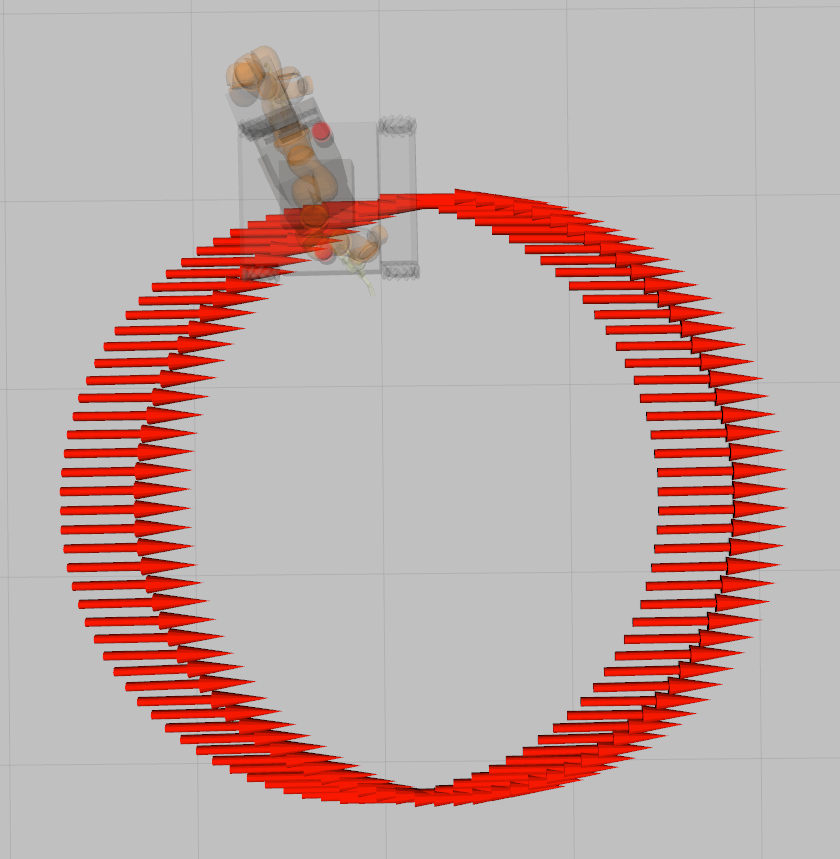
\includegraphics[width=\linewidth]{imgs/wstepne_badania/circle.png}
			\caption{ruch po okręgu ze stałą orientacją względem świata}
			\label{fig:tf}
		\end{figure}

		Kierunek strzał oznacza, że orientacja bazy podczas ruchu nie ulegała zmianie, natomiast wszystkie punkty układają się w pełen okrąg.
		
		Następnym testem, który został przeprowadzony, był test planera globalnego i lokalnego udostępnionych razem z platformą.
		Ze względu na nacisk położony na holonomiczny ruch bazy poświęciłem więcej uwagi algorytmowi planowania lokalnego, plan globalny był jedynie weryfikowany przez sprawdzenie, czy została wytyczona ścieżka.
		Zadaniem robota było przejechanie z punktu o współrzędnych $[1.0 ,2.0]$ do współrzędnych $[2.0, 0.0]$.
		

		\begin{figure}[h!]
 			 \centering
  			\begin{subfigure}[b]{0.4\linewidth}
   				 \includegraphics[width=\linewidth]{imgs/wstepne_badania/plan.png}
    				\caption{plan globalny i lokalny}
  			\end{subfigure}
  			\begin{subfigure}[b]{0.4\linewidth}
    				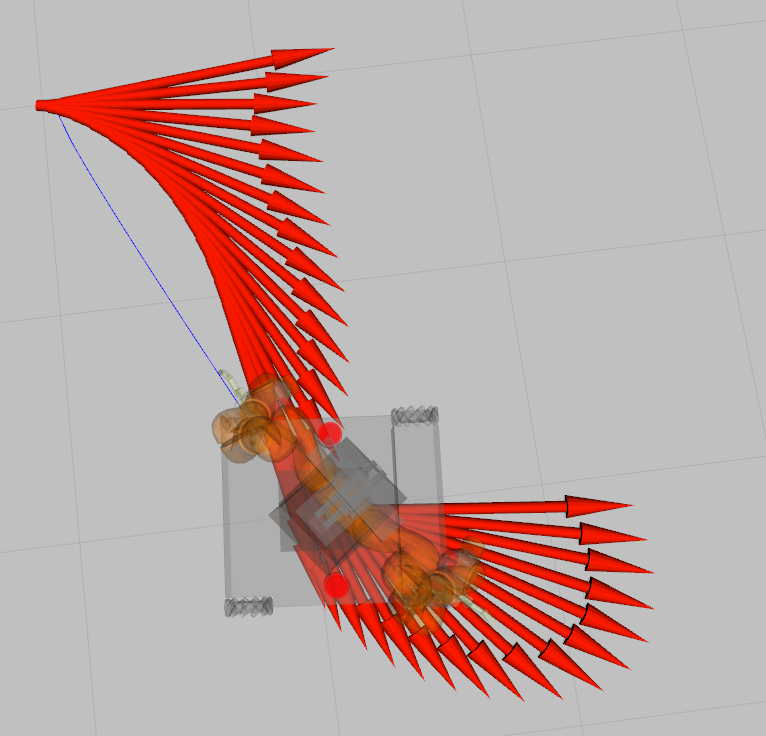
\includegraphics[width=\linewidth]{imgs/wstepne_badania/path.png}
   				 \caption{trajektoria ruchu}
  			\end{subfigure}
  			\caption{The same cup of coffee. Two times.}
 			 \label{fig:plan}
		\end{figure}

		Na pierwszym rysunku z \ref{fig:plan} pokazano, jak plan globalny prawidłowo wyznaczył najkrótszą ścieżkę do punktu docelowego. 
		Natomiast ścieżka algorytmu lokalnego pokazuje, że robot jest traktowany jako baza różnicowa, co ostatecznie dowodzi trajektoria ruchu widoczna na drugiej ilustracji.
		
	\subsection{Budowanie mapy}
		
		W obecnej chwili do budowy mapy można wykorzystywać jedynie pojedynczy czujnik laserowy znajdujący się po lewej lub po prawej stronie bazy jezdnej.
		Jest również zaimplementowana projekcja mapy zajętości generowanej przez kamerę Kinect na płaszczyznę dwuwymiarową, jednak nie została jeszcze ona zintegrowana z modułem odpowiedzialnym za tworzenie map statycznych, na chwilę pisania tego rozdziału budowanie mapy opiera się tylko na pojedymczym skanerze laserowym.
		Na ilustracjach \ref{fig:scan} pokazano, jak na mapę lokalną został zrzutowany fragment wystającego blatu stolika.
			
			
		\begin{figure}[h!]
 			 \centering
  			\begin{subfigure}[h]{\linewidth}
   				 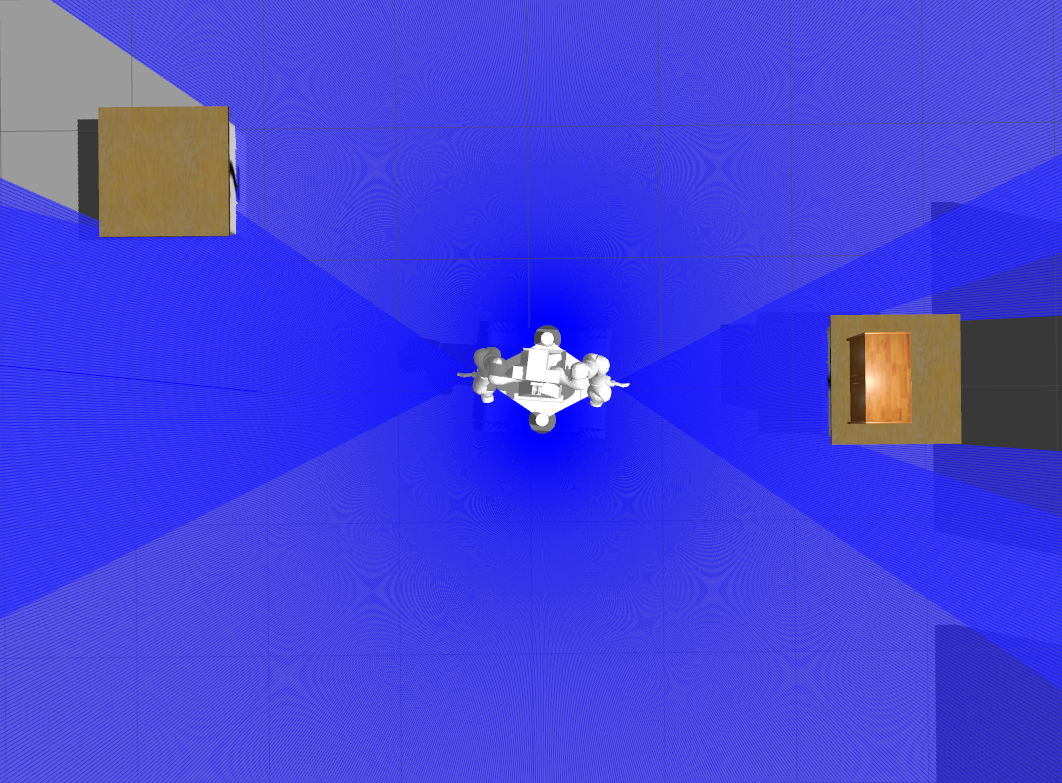
\includegraphics[width=\linewidth]{imgs/wstepne_badania/gazebo_scan.png}
    				\caption{plan globalny i lokalny}
  			\end{subfigure}
  			\begin{subfigure}[h]{\linewidth}
    				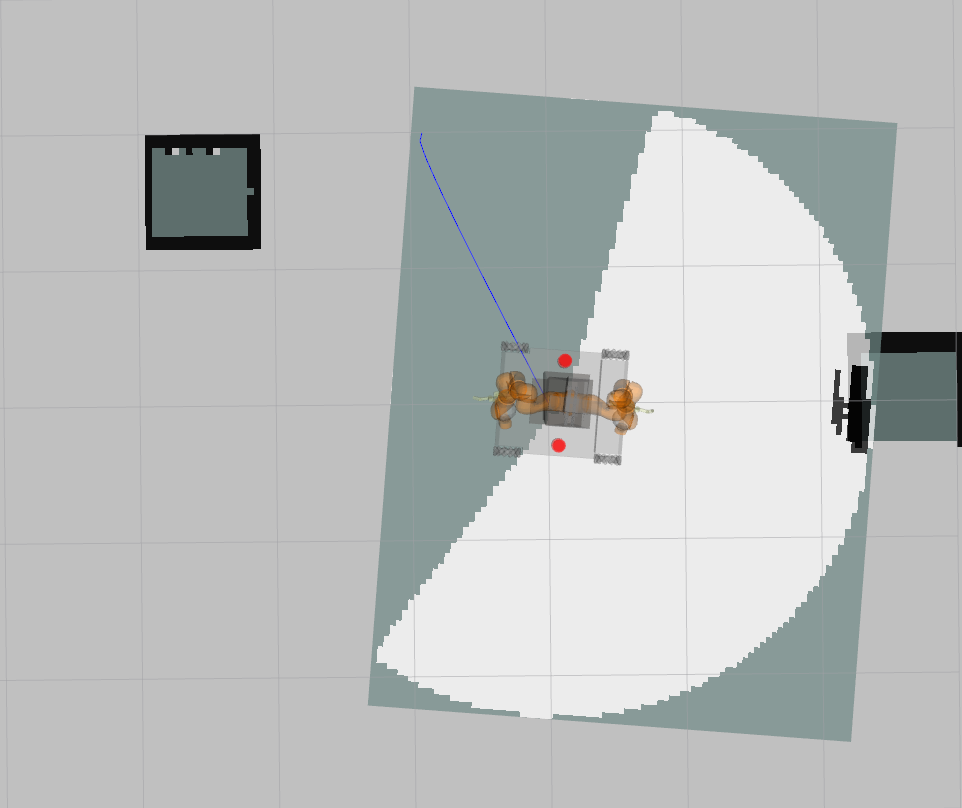
\includegraphics[width=\linewidth]{imgs/wstepne_badania/rviz_scan.png}
   				 \caption{trajektoria ruchu}
  			\end{subfigure}
  			\caption{rzutowanie skanu kamery Kinect}
 			 \label{fig:scan}
		\end{figure}
	
		Na rysunku \ref{fig:mapping} przedstawiono pojedynczy skan laserowy wykonany w nieznanym środowisku przed poruszeniem bazą robota. 

		\begin{figure}[h!]
 			 \centering
  			\begin{subfigure}[b]{0.4\linewidth}
   				 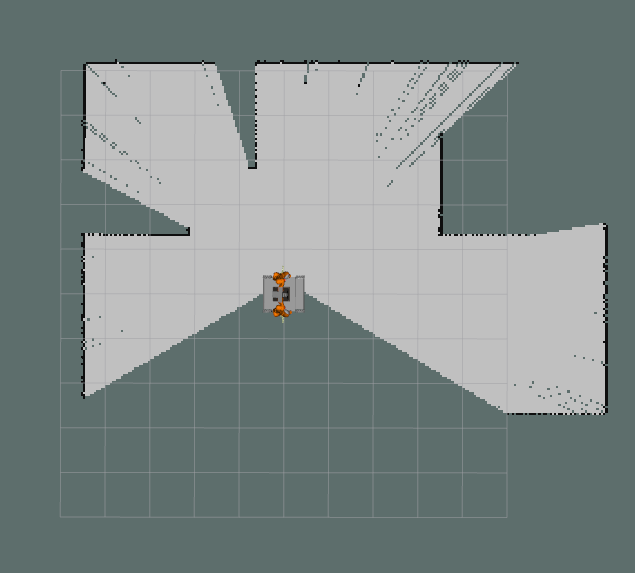
\includegraphics[width=\linewidth]{imgs/wstepne_badania/scan_l.png}
    				\caption{lewy skaner}
  			\end{subfigure}
  			\begin{subfigure}[b]{0.4\linewidth}
    				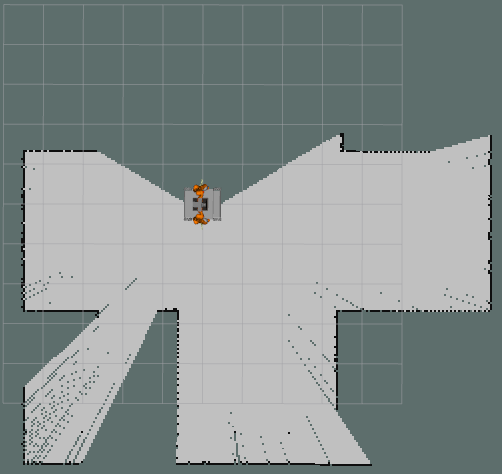
\includegraphics[width=\linewidth]{imgs/wstepne_badania/scan_r.png}
   				 \caption{prawy skaner}
  			\end{subfigure}
			\begin{subfigure}[b]{0.9\linewidth}
    				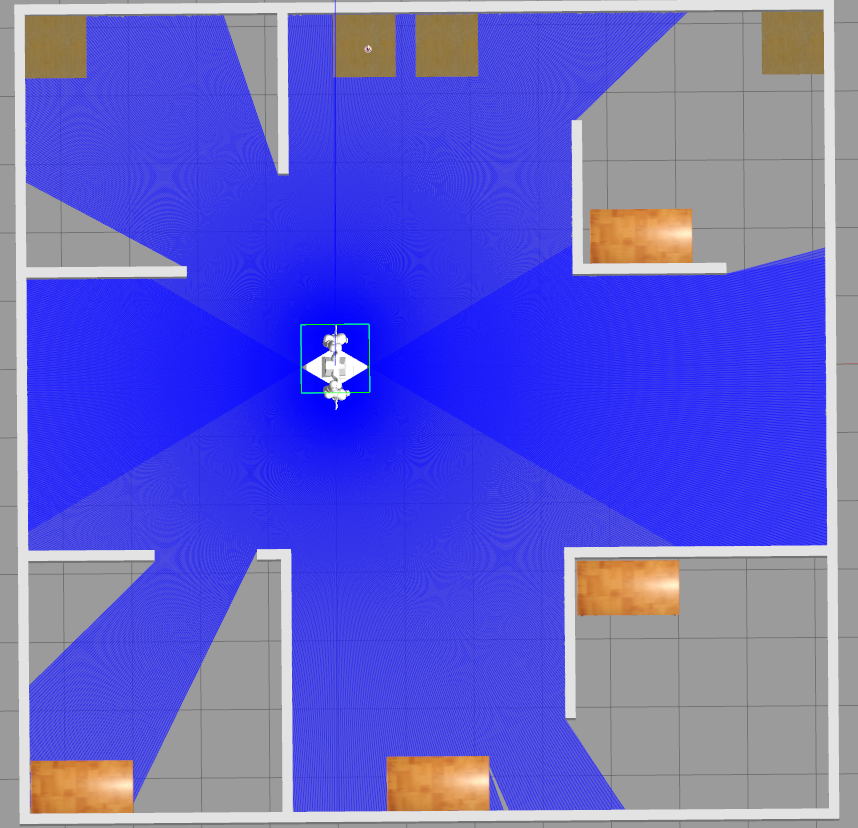
\includegraphics[width=\linewidth]{imgs/wstepne_badania/scan_all.png}
   				 \caption{pokrycie obydwu skanerów}
  			\end{subfigure}
  			\caption{pokrycie przestrzeni}
 			 \label{fig:mapping}
		\end{figure}

	
		Podczas próby przetestowania modułu \textit{gmapping} wykorzystującego pojedynczy skaner laserowy do zbudowania statycznej mapy zajętości okazało się, że w systemie znajdują się błędy uniemożliwiające budowę mapy. 
		Na rysunku \ref{fig:tf} ukazane zostało drzewo transformacji, na którym widać, że pierwotnym układem współrzędnych jest \textit{odom}, z którego następnie jest przeliczana transformacja na układ \textit{world}, a z tego równolegle na \textit{torso\_base} oraz równolegle \textit{map}. 
		Jest to błędna struktura, poprawna posiada \textit{world} jako pierwotny układ współrzędnych, od niego przechodzi transformacja do układu \textit{map}, stąd do \textit{odom}, a wreszcie do \textit{torso\_base}, bez rozgałęzień. 
		
		\begin{figure}
			\centering
			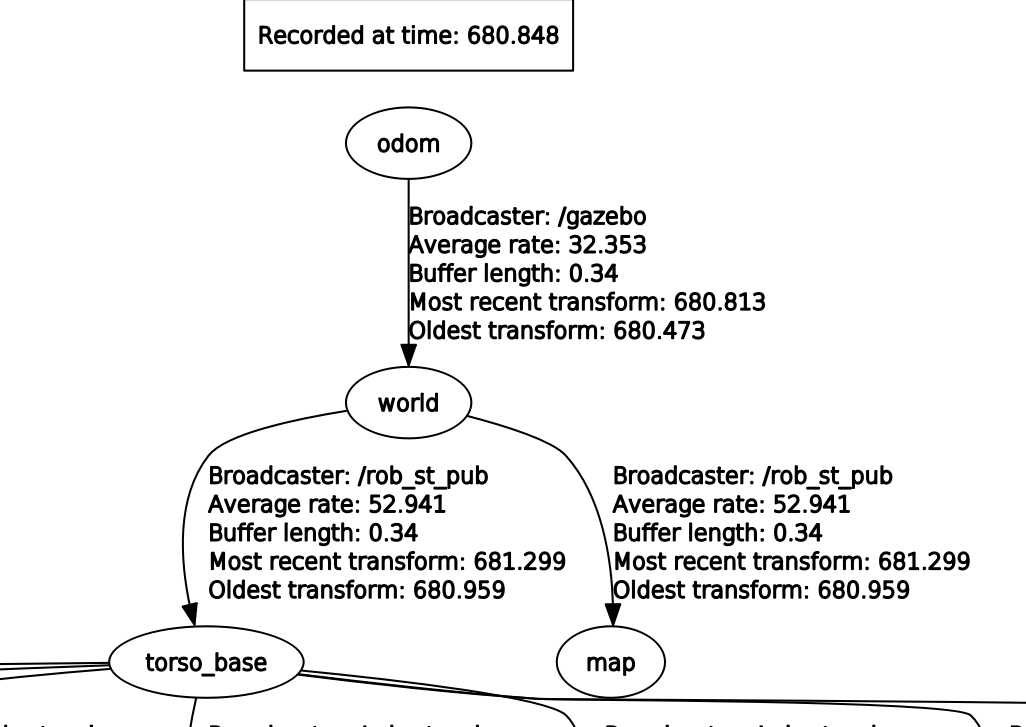
\includegraphics[width=\linewidth]{imgs/wstepne_badania/tf.png}
			\caption{błędne drzewo transformacji}
			\label{fig:tf}
		\end{figure}
		
		
	
	\subsection{lokalizacja}
	
		Ta część badań jest ściśle zależna od budowania mapy oraz poprawności drzewa transformacji.
		Dopóki ten element wykazuje błędne działanie, lokalizacja robota z pomocą odometrii oraz laserów i kamery Kinect, ale też wysyłanie pozycji innych przedmiotów w jego otoczeniu jest niemożliwa.
		Dlatego ta część badań zostaje wstrzymana do czasu usunięcia błędów w drzewie transformacji. 
		Na rysunku ... ukazano próbę jednoczesnej lokalizacji i budowania mapy robota przy opisanym stanie systemu. 
		Robot jechał ze stałą prędkością $0.4$ w kierunku \textit{x} bazy i przejechał w rzeczywistości około $6$ metrów.
		
		\begin{figure}
			\centering
			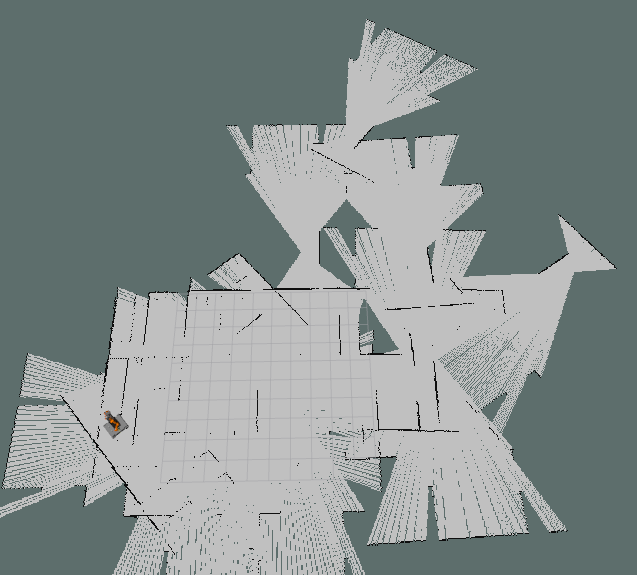
\includegraphics[width=\linewidth]{imgs/wstepne_badania/crazy.png}
			\caption{błąd w dynamicznym tworzeniu mapy statycznej i w lokalizacji}
			\label{fig:tf}
		\end{figure}
		
		
		


%		\begin{figure}[h]
%			\centering
%			\begin{subfigure}[b]{0.4\linewidth}
 %				 \includegraphics[0.8\linewidth]{imgs/wstepne\_badania/plan.png}
%				  \caption{Plan globalny i plan lokalny }
%				  \label{fig:plan}
%			  \end{subfigure}
%			\begin{subfigure}
% 				 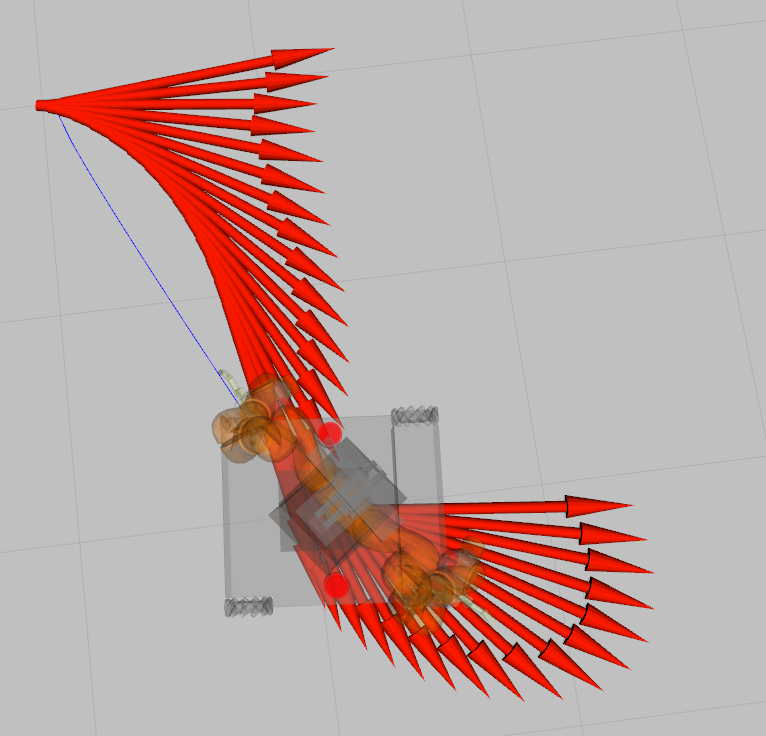
\includegraphics[width=0.8\linewidth]{imgs/wstepne_badania/path.png}
%				  \caption{Plan globalny i plan lokalny }
%				  \label{fig:path}
%			  \end{subfigure}
%		\end{figure}

 %TODO

	
	
	%Podsumowanie
	\chapter{Plan Działania}

plan %TODO
	
	Bibliografia dla mnie:

\bibliographystyle{apacite}
\bibliography{References}%wip

	
		
\end{document}
